\cleardoublepage
\section{文献综述}

\subsection{背景介绍}
\subsubsection{概要}
在普适计算与物联网（IoT）飞速发展的时代背景下，人机交互（HCI）模式正经历着从传统的物理接触式向自然非接触式的深刻变革。传统的交互终端，如多点触控屏幕、物理按键及鼠标，虽然在精度和响应速度上已趋于成熟，但在诸多特定应用场景中表现出局限性\cite{6177682}。例如，在医疗手术室、无尘车间或驾驶舱等环境中，物理接触不仅可能带来卫生隐患，还可能分散操作者的注意力，降低工作效率 。随着增强现实（AR）、虚拟现实（VR）以及智能座舱等技术的不断演进，用户对于更直观、更自由、更符合人类表达直觉的交互方式提出了更高要求。手势识别作为人类非语言交流的核心组成部分，因其具备跨越语言障碍、支持隐蔽操作及高自由度表达等特性，已成为下一代人机交互接口的研究焦点\cite{mainpaper} 。

手势识别技术路线主要分为视觉传感、穿戴式传感与射频传感三类。以摄像头为核心的视觉方案虽然在图像识别领域取得了显著突破，但其高度依赖光照强度，且在暗光环境、视距（LoS）遮挡及涉及用户私密空间的场景中，面临严重的性能衰减与隐私泄露风险。穿戴式方案如数据手套、肌肉电信号（sEMG）传感器及惯性测量单元（IMU），虽能提供厘米级的运动追踪精度，但其物理束缚感、繁琐的佩戴流程以及高昂的设备维护成本，限制了其在普通消费电子领域的普及\cite{werable}。相比之下，基于微波与毫米波（mmWave）的多普勒雷达传感技术，凭借其全天候工作、穿透遮挡能力及天然的隐私保护优势，展现出极高的学术价值与应用潜力\cite{soli}。

雷达传感器通过主动发射电磁波并接收目标反射的回波，能够捕捉目标在微米至厘米级别的微波波动 。多普勒效应作为其核心物理机制，将手部及手指的复杂运动转化为回波信号中的频率偏移与相位调制。近年来，随着半导体制造工艺向 28nm 及更深纳米级演进，毫米波雷达芯片正朝着超大规模集成（SoC）、低功耗及微型化方向跨越式发展 。Google 的 Soli 项目首次展示了将 60GHz 调频连续波（FMCW）雷达集成于智能手机的可行性，标志着雷达手势识别从军事、气象等领域正式跨入个人终端消费市场\cite{rs13030527} 。我们综合讨论近些年来的主流手势识别技术的核心性能指标如表\ref{tab:sensor_comparison}。

\begin{table}[htbp]
    \centering
    \renewcommand{\arraystretch}{1.5}
    \caption{\bfseries 各类传感技术评估维度对比}
    % 使用 m{宽度} 实现垂直居中，>{\centering\arraybackslash} 实现水平居中
    \begin{tabular}{|>{\centering\arraybackslash}m{1.6cm}|>{\centering\arraybackslash}m{2.1cm}|>{\centering\arraybackslash}m{2.1cm}|>{\centering\arraybackslash}m{2.1cm}|>{\centering\arraybackslash}m{2.1cm}|>{\centering\arraybackslash}m{2.1cm}|}
    \hline
    \textbf{评估维度} & \textbf{多普勒雷达 (mmWave)} & \textbf{计算机视觉 (RGB-D)} & \textbf{惯性传感器 (Wearable)} & \textbf{超声波/声学感知} & \textbf{Wi-Fi CSI 感知} \\ \hline

    \textbf{隐私安全性} & \textbf{极高}：无图像、无生物识别信息 & \textbf{低}：存在面部及隐私环境泄露风险 & \textbf{中}：仅运动数据，但需数据存储 & \textbf{高}：声波无法还原图像 & \textbf{高}：射频信号难以直观解读 \\ \hline

    \textbf{环境适应性} & \textbf{极强}：不受光照、烟雾、遮挡影响 & \textbf{弱}：光照敏感，视距受限 & \textbf{强}：不受外界环境干扰 & \textbf{中}：受环境噪声和气流影响 & \textbf{强}：支持穿墙探测 \\ \hline

    \textbf{佩戴便捷性} & \textbf{免佩戴}：真正的非接触式交互 & \textbf{免佩戴} & \textbf{差}：需要物理接触，舒适度低 & \textbf{免佩戴} & \textbf{免佩戴} \\ \hline

    \textbf{分辨率/精度} & \textbf{高}：可捕捉亚毫米级微动 & \textbf{极高}：像素级几何形状识别 & \textbf{极高}：高精度采样 & \textbf{中}：依赖声速，动态响应慢 & \textbf{低}：通常为厘米级粗糙识别 \\ \hline

    \textbf{硬件成本} & \textbf{中等}：由于CMOS集成度提高持续下降 & \textbf{低}：手机摄像头普及 & \textbf{中-高}：需额外硬件 & \textbf{极低}：利用现有麦克风/扬声器 & \textbf{极低}：复用路由器硬件 \\ \hline
    \end{tabular}
    \label{tab:sensor_comparison}
\end{table}

与此同时，随着人工智能技术（Artificial Intelligence, AI）的迅猛发展，更多智能终端在传统的用户交互的基础上，集成了多种传感器和智能算法，实现了更为复杂和智能化的交互方式。在当下的分类和预测任务中神经网络（Neural Network）能够处理图像、语音和文本等高度非线性的原始数据，并将其映射到预定义的类别中,例如:多层感知机（MLP） 作为基础架构，通过全连接层对结构化数据（如用户画像、财务指标）进行特征组合，实现精准的二分类或多分类\cite{Taud2018MultilayerP};卷积神经网络（CNN）在图像识别和目标检测领域表现卓越,它通过卷积核提取空间特征，能够自动识别复杂的视觉模式，用于人脸识别、医疗影像诊断等领域\cite{kim-2014-convolutional}\cite{CNNreview}。循环神经网络（RNN）及其变体（LSTM/GRU）专注于序列分类，能够捕捉文本或语音中的上下文语义\cite{RNNreview}。

\subsubsection{问题建模}

该系统由两个核心部分组成：雷达数据采集部分与神经网络识别部分。整体流程通过嵌入式处理器/MCU进行统筹管理。示意图见\ref{fig:brief}。
数据采集部分使用毫米波天线阵列（mmWave Antenna Array）向空间发射电磁波信号。当手部进行动态动作时，电磁波发生反射，由接收天线（Rx）捕捉回波信号。回波信号首先经过模拟前端。主要包括利用低噪声放大器（LNA）对微弱回波进行放大，并通过混频器（Mixers）进行下变频处理。处理后的模拟信号通过模数转换器（ADC）转化为数字信号，进入数字处理阶段。随后在神经网络处理阶段原始数字信号被转化为神经网络可理解的高维特征，提取出的特征（如RDM和微多普勒谱图）被送入分类器模型，系统输出识别结果（如"滑动"、"推"等动作标识），并触发相应的指令响应。

\begin{figure}[H]
    \centering
    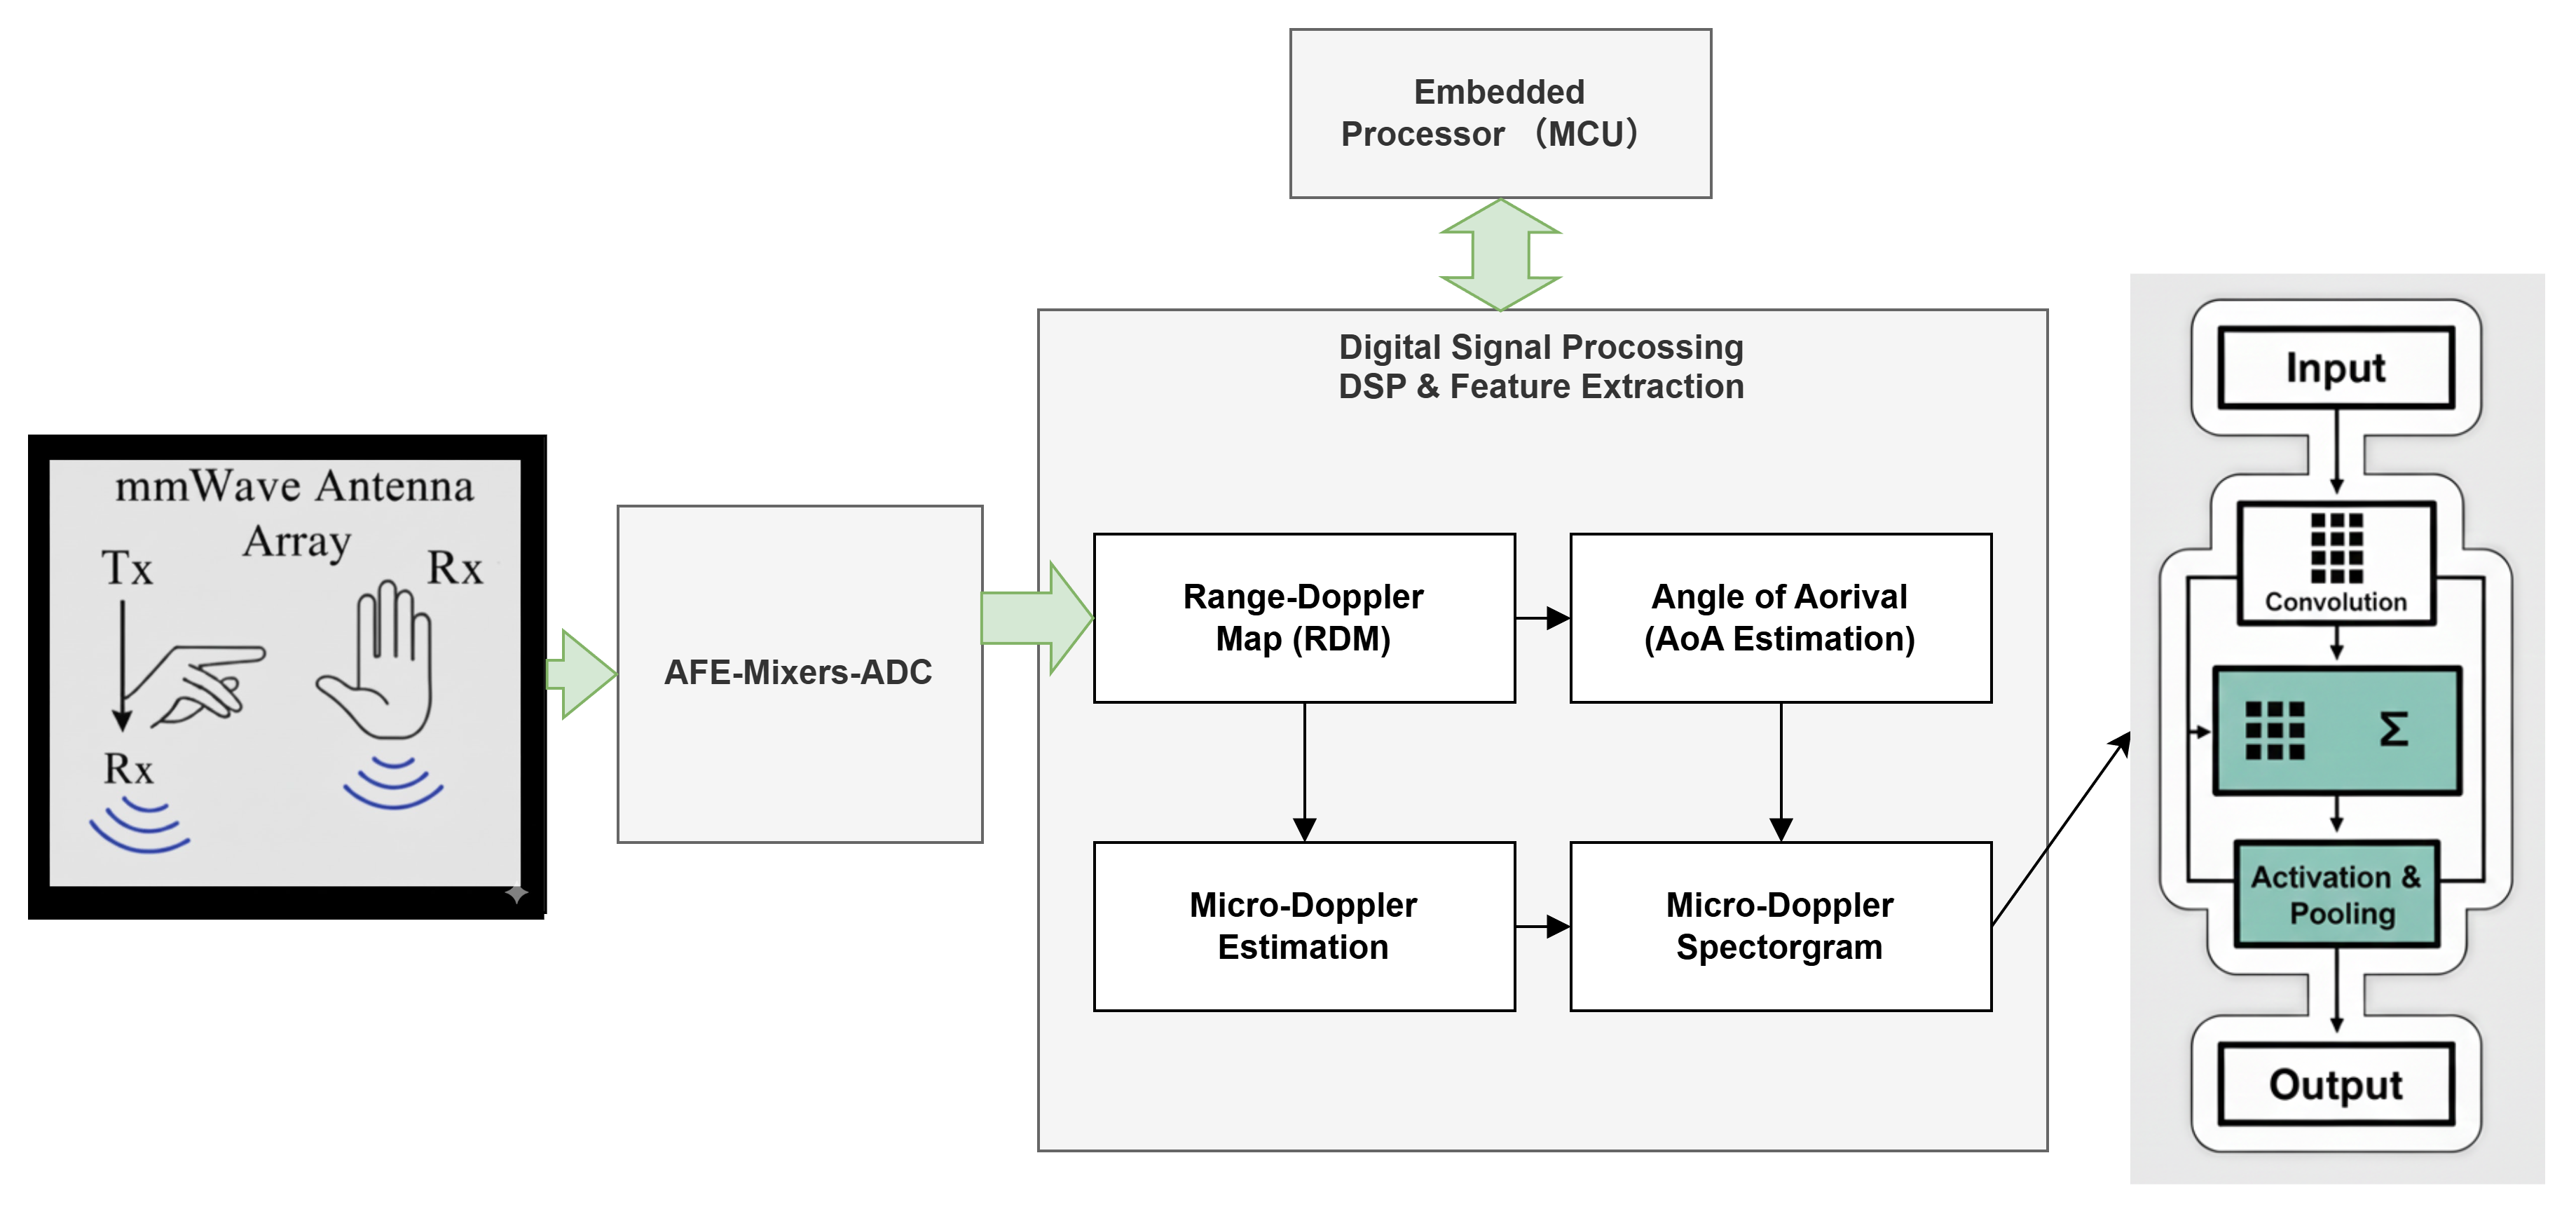
\includegraphics[width=\textwidth]{doc_3in1/figs/01/image.png}
    \caption{基于Doppler雷达的手势识别系统示意图}
    \label{fig:brief}
\end{figure}

\paragraph{雷达数据采集}
多普勒雷达手势识别的物理基石在于多普勒效应，即当波源与观察者之间存在相对运动时，观察者接收到的波频率发生改变的现象。在雷达手势感知中，这一效应被精细地用于刻画手部动力学特征。单频连续波（CW）雷达是实现多普勒检测最基础的体制。其发射信号通常表现为单频正弦波：
\begin{equation}
s_T(t) = A_T \cos(2\pi f_c t + \phi(t))
\end{equation}

其中，$f_c$ 为载波频率，$\phi(t)$ 代表发射机振荡器的相位噪声。当电磁波照射到距离雷达 $d(t)$ 的手部目标并发生反射后，接收机获取的回波信号 $s_R(t)$ 经过往返时延 $\tau(t) = 2d(t)/c$ 产生相位偏移：
\begin{equation}
s_R(t) = A_R \cos(2\pi f_c (t - \tau(t)) + \phi(t - \tau(t)))
\end{equation}

在接收前端，回波信号与发射信号的采样样本进行混频（Mixer）并经过低通滤波，产生基带信号。对于一个以径向速度 $v$ 匀速运动的目标，其产生的时间变动相位项导出多普勒频移 $f_D$：
\begin{equation}
f_D = -\frac{2v}{\lambda} = -\frac{2v f_c}{c}
\end{equation}

公式表明，多普勒频移与目标的运动速度成正比，与载波波长成反比。由于毫米波雷达的波长极短（例如 60GHz 对应波长为 5mm），即使是微小的手指抖动（速度 $v$ 极小）也能激发出显著的频率偏移，这奠定了其捕捉微细手势（Micro-gestures）的物理基础。

尽管单频 CW 雷达能精确测量速度，但其缺乏测距能力，且无法区分处于相同速度的多个目标。调频连续波（FMCW）体制通过对载波进行线性扫频解决了这一问题。其发射频率在周期 $T_c$ 内随时间线性增加，带宽为 $B$。回波信号与发射信号之间的差频信号（拍频信号）频率 $f_{beat}$ 包含了目标的距离信息：


\begin{equation}
f_{beat} = \frac{2d}{c} \cdot \frac{B}{T_c}
\end{equation}

通过对接收到的数字中频（IF）数据流执行二维 FFT 处理，可以生成距离-多普勒图（Range-Doppler Map, RDM）。在 RDM 中，横轴通常代表目标的径向速度，纵轴代表距离，从而实现了在距离-速度平面的目标分离 。此外，引入单输入多输出（SIMO）或多输入多输出（MIMO）天线阵列，利用各接收通道间的空间相位差，可以进一步解算出目标的方位角与俯仰角。多维感知能力的提升使得雷达不仅能识别手势的类别，还能实时重构手部在三维空间中的运动轨迹。

\paragraph{神经网络建模}

收集得到的信号后，需要经过分类任务对应相应的动作行为，这一步通过一个神经网络 （Neural Network）的建模实现。在多普勒雷达手势识别任务中，神经网络被建模为一个复杂的非线性映射函数 $f_\theta(\cdot)$。其核心目标是学习从高维雷达信号特征空间 $\mathcal{X}$（如 Range-Doppler Map 或 Micro-Doppler Spectrogram）到离散手势标签空间 $\mathcal{Y}$ 的映射关系。

假设输入特征向量为 $\mathbf{x} \in \mathbb{R}^n$，一个具有 $L$ 层的深度神经网络可以表示为一系列嵌套的非线性变换：
\begin{equation}
    \hat{\mathbf{y}} = f_\theta(\mathbf{x}) = \sigma_L \left( \mathbf{W}_L \sigma_{L-1} \left( \dots \sigma_1 \left( \mathbf{W}_1 \mathbf{x} + \mathbf{b}_1 \right) \dots \right) + \mathbf{b}_L \right)
\end{equation}
其中，$\theta = \{\mathbf{W}_l, \mathbf{b}_l\}_{l=1}^L$ 代表网络的可学习参数集合，$\mathbf{W}_l$ 为权重矩阵，$\mathbf{b}_l$ 为偏置向量，$\sigma(\cdot)$ 为非线性激活函数（如 ReLU、Leaky ReLU 或 Sigmoid）。

神经网络的训练本质上是一个经验风险最小化（Empirical Risk Minimization, ERM）的优化过程。通过定义损失函数 $\mathcal{L}(\hat{\mathbf{y}}, \mathbf{y})$ 来衡量模型预测值与真实标签之间的偏差。在多分类手势识别任务中，通常采用交叉熵损失函数（Cross-Entropy Loss）：
\begin{equation}
    \mathcal{J}(\theta) = -\frac{1}{N} \sum_{i=1}^N \sum_{k=1}^K y_{i,k} \log(\hat{y}_{i,k}) + \frac{\lambda}{2} \|\theta\|^2_2
\end{equation}

其中 $N$ 为样本总数，$K$ 为手势类别数，$\lambda$ 为正则化系数用于防止模型过拟合。参数更新过程遵循梯度下降法（Gradient Descent）：
\begin{equation}
    \theta_{t+1} = \theta_t - \eta \cdot \nabla_\theta \mathcal{J}(\theta_t)
\end{equation}

其中 $\eta$ 为学习率，$\nabla_\theta \mathcal{J}(\theta_t)$ 为损失函数关于参数的偏导数，通过反向传播算法\cite{rumelhart1986learning}（Backpropagation）计算获得。

对于 $K$ 类手势识别任务，网络末端通常接入 Softmax 层，将隐藏层的输出映射为各类别的概率预测分布 $P(y=k|\mathbf{x})$：
\begin{equation}
    P(y=k|\mathbf{x}) = \frac{e^{z_k}}{\sum_{j=1}^K e^{z_j}}
\end{equation}

其中 $z_k$ 是分类层对第 $k$ 类的原始输出评分（Logit）。最终的预测结果由最大后验概率（MAP）准则决定：
\begin{equation}
    \text{Label} = \arg\max_{k \in \{1, \dots, K\}} P(y=k|\mathbf{x})
\end{equation}

在测试阶段，模型参数 $\theta$ 被冻结，不再进行更新。模型通过前向推断（Inference）对未见过的测试集 $\mathcal{D}_{test}$ 进行泛化能力评估。核心评价指标为分类准确率（Accuracy）：
\begin{equation}
    \text{Accuracy} = \frac{1}{|\mathcal{D}_{test}|} \sum_{x_i \in \mathcal{D}_{test}} \mathbb{I}(f_\theta(x_i) = y_i)
\end{equation}

其中 $\mathbb{I}(\cdot)$ 为指示函数，当预测标签与真实标签一致时取值为 1，否则为 0。

\subsection{国内外研究现状}

\subsubsection{研究方向及进展}
早期的雷达手势识别系统受限于硬件带宽与天线数量，主要依赖于一维信号特征。主要关注幅度随时间的变化（Time-Amplitude）或幅度随距离的变化（Range-Amplitude）。高分辨率距离像（High-Resolution Range Profile, HRRP）是这一阶段的核心\cite{1453769}。它通过宽频带信号处理，获取目标在雷达射线方向上的散射点分布，反映目标的径向结构特征。与此同时1D 特征无法区分处于相同距离但不同方位角的目标（如手部与躯干），在复杂环境下极易产生目标混叠 。

随着调频连续波（FMCW）技术的成熟，2D 建模成为了手势识别的经典范式。通过对回波执行二维 FFT 处理，将信号映射为距离-多普勒平面（Range-Doppler Map, RDM），同时解算出目标的径向距离与径向速度。RDM 能够有效分离动态手部与静态背景杂波,在此基础上，通过短时傅里叶变换（STFT）提取出的微多普勒（micro-Doppler）指纹，能够精细刻画手指屈伸等细微动作产生的频率调制\cite{1603402}。

4D 建模是目前最前沿的技术方向，它标志着雷达从"探测传感器"向"高分辨率成像仪"的转变。维度定义：4D 指的是距离（Range）、径向速度（Doppler/Velocity）、方位角（Azimuth）以及俯仰角（Elevation/Height）。生成包含三维空间坐标与实时速度信息的密集点云（Point Cloud）,每个点云点通常携带 $(x, y, z, v, I)$ 等五个维度的数据，其中 $I$ 为反射强度。4D 建模引入了俯仰角信息，在一定程度上解决了 3D 雷达无法区分"高处障碍物（如桥梁）"与"路面目标（如车辆）"的痛点。在手势识别中，4D 建模支持对复杂 3D 运动轨迹（如空中连续写字）的高保真重构，其点云密度与精度已接近低线束 LiDAR 性能。

全球雷达手势识别的研究热潮很大程度上源于 2016 年 Google 推出的 Project Soli。这一里程碑式的项目首次证明了利用 60 GHz 调频连续波（FMCW）雷达捕捉指尖微小动作的可能性。通过集成天线阵列与随机森林等机器学习算法，Soli 实现了对诸如"拨动转盘"、"摩擦手指"等复杂微动作的精准识别，其追踪精度达到了亚毫米级别。此后，国际半导体巨头如英飞凌（Infineon）、德州仪器（TI）和意法半导体（ST）纷纷跟进，推出了集成了硬件加速器（HWA）和微控制器（MCU）的毫米波雷达 SoC 芯片。

在学术界，欧洲的研究机构如英飞凌、卡尔斯鲁厄理工学院（KIT）和比利时微电子研究中心（imec）在低功耗雷达架构和少样本学习（Few-shot Learning）领域占据前沿\cite{withmetaL}\cite{9722880}。例如，imec 致力于开发亚毫瓦级的脉冲雷达，在IEEE RFIC 2020 会议上展示了集成在标准28nm CMOS中的60GHz毫米波运动检测雷达。超灵敏雷达可实现2厘米的距离分辨率，针对生命体征监测和手势识别进行了优化，具有5米处心跳检测以及对行人位置和速度的精确跟踪的能力。紧凑型雷达芯片仅消耗62mW\cite{imec}。国际研究的重点已从早期的"单纯识别"转向"实时性、低功耗与泛化能力的平衡"，强调在嵌入式平台上实现毫秒级的响应延迟 。

此外，国外研究针对标注雷达数据昂贵的问题，研究人员开始利用扩散模型（Diffusion Models）生成高度逼真的合成多普勒指纹，并结合物理建模缩短"仿真到现实"的差距（Sim-to-Real Gap）\cite{wu2024cross}；mmWrite 等系统利用大规模相控阵雷达实现毫米级的指尖追踪，支持在任意平面上进行虚拟手写，并结合双向 LSTM（Bi-LSTM）进行字符识别，识别准确度突破 98\% \cite{regani2021mmwrite}。

2025年第三季度发布的论文中提出在一个闭环系统中，雷达接收机对环境进行感知，学习目标与背景的相关信息，并根据预设任务目标自适应地调整发射机参数 。尽管这一范式在频谱共享、目标检测与跟踪领域已取得显著进展，但在针对手势控制和智能环境交互的应用中，如何根据用户的即时状态调整雷达的物理层参数仍是一个相对空白的领域 。Gurbuz et al.等人首个将发射信号的自适应性与人类用户交互状态直接挂钩的研究工作 。通过引入"人机在环"（Human-in-the-Loop）机制，雷达不再只是一个被动的数据采集器，而是一个能够理解交互上下文并主动优化其感知策略的智能实体 \cite{Gesture-basedHuman-in-the-LoopInteractionwithFully-AdaptiveRadar}。

中国在雷达手势识别领域展现出极强的后发优势，重点集中在算法层面的创新与特定场景的应用落地。《雷达学报》近期刊载了关于超宽带雷达人体动作四维成像数据集的研究，为国产雷达手势识别算法提供了核心基石；北京理工大学团队探讨了基于 Transformer 位置编码与序列编码的多帧 RDM 特征融合算法，强调了多维特征融合优于单特征识别的结论。

北京理工大学、南京邮电大学、清华大学以及电子科技大学等高校构成了研究的主力军。国内研究者敏锐地观察到雷达信号在高维特征利用上的冗余问题，提出了多种时空压缩特征表示学习方法。例如，南京邮电大学团队开发的毫米波雷达手势识别算法，通过对 FMCW 信号进行时空压缩特征提取，有效解决了深度学习模型在处理大规模原始雷达数据时的计算瓶颈\cite{chong2022millimeter}。针对微小动作识别难的问题，国内学者提出了诸如 CQ-MobileNetV3 的轻量化网络结构，通过引入注意力机制（CBAM）和自注意力模块，在仅需 0.027 GFLOPs 计算量的情况下实现了极高的识别准确率\cite{CQ} 。此外，国内研究在雷达与视觉融合、身份识别联合手势识别等方面也取得了重要进展，通过 Gram 匹配等损失函数优化，显著提升了跨场景的鲁棒性\cite{shin2024methodological}。

表\ref{tab:model_comparison}对比了近三年出现的几种轻量化手势识别网络的参数量、功耗性能和应用领域。可以看出在雷达采样之外，特定的神经网络和模型架构能够有效地提升识别任务的多样性，同时也会带来一定的计算资源负载。

\begin{table}[htbp]
    \centering
    \renewcommand{\arraystretch}{1.5}
    \caption{\bfseries 手势识别模型与系统性能对比}
    % 根据原图5列调整列数和宽度分配
    \begin{tabular}{|>{\centering\arraybackslash}m{2.5cm}|>{\centering\arraybackslash}m{3cm}|>{\centering\arraybackslash}m{2cm}|>{\centering\arraybackslash}m{2cm}|>{\centering\arraybackslash}m{3cm}|}
    \hline
    \textbf{模型名称} & \textbf{核心架构} & \textbf{参数量} & \textbf{功耗/延迟} & \textbf{识别任务} \\ \hline

    \textbf{CQ-Mobile NetV3} & 优化的 MobileNet + CBAM & 0.207 M & 27 MFLOPs & 14类微手势 \\ \hline

    \textbf{TinyRadar NN\cite{9381994}} & 2D CNN + TCN & 46 K & 120 mW & 11类通用手势 \\ \hline

    \textbf{RadarNet\cite{yang2020radarnet}} & Multi-head 2D CNN + LSTM & - & < 1 s & 左右/上下扫动手势 \\ \hline

    \textbf{No-ML System} & 纯 DSP (FFT + Azimuth) & N/A & < 10 ms & 滑动、推压 \\ \hline
    \end{tabular}
    \label{tab:model_comparison}
\end{table}

\subsubsection{存在问题}

虽然基于毫米波的手势识别已经取得了非常多的研究进展与应用，其仍存在以下几个关键问题和挑战

\begin{enumerate}
    \item \textbf{现实噪音扰动：}在实际复杂的室内人机交互场景中，目标手部并非处于孤立的真空中。人体躯干由于其巨大的反射面积（RCS），其回波强度通常比指尖运动回波高出 20-30 dB。这种极大的动态范围差异对 ADC 采样位数提出了严苛要求。更具挑战性的是，躯干的微小晃动或呼吸诱发的低频分量，在进行离散傅里叶变换（DFT）时，会由于窗函数的非周期性截断产生严重的频谱泄漏（Spectral Leakage），使得低频能量向高频区间扩散，从而像'迷雾'一样掩盖了代表微手势特征的高频微弱多普勒分量。
    \item \textbf{毫米波散射：}在 2021 年发表于 IEEE Transactions on Microwave Theory and Techniques 的关键论文中，Zhang 及其合作者指出，目前主流的微多普勒识别方法存在严重的鲁棒性缺陷 。手部作为电磁波的散射体，其尺寸与毫米波波长处于同一数量级，属于复杂的 Mie 散射区 \cite{mainpaper}。这意味着即使是同一个手势，由于手掌大小、手指曲率以及相对于雷达的入射角微小差异，回波产生的频谱纹理（Spectrogram）也会发生显著且不规则的变化,这导致不同照射角度、不同用户生理特征下的回波相位分布极不规则，极大地限制了传统线性重建算法的鲁棒性 。
    \item \textbf{神经网络算法限制：}"黑盒"深度学习方案具有样本依赖性：许多基于 CNN 或 RNN 的方法直接将时频图喂入模型。虽然识别率高，但通常需要数以万计的标记数据来覆盖不同用户的生理差异和执行风格。这对于个人便携式设备而言，训练成本过高，且模型泛化能力受限于数据集质量。并且基于深度学习的分类器通常在特定数据集上表现优秀，但在面对未见过的（untaught）新用户或新环境（如不同材质遮挡、不同距离/角度）时，识别准确率往往会大幅下降。
    \item \textbf{存储和计算负载：}高维雷达数据（如 4D 点云或 RDM 序列）具有极大的冗余和计算负载。在内存和功耗受限的嵌入式 IoT 设备或移动终端上，运行复杂的 3D-CNN 或变体网络会面临严重的延迟问题。对于极高的雷达数据采样率（通常每秒数千个 Chirp），目前的主流做法是进行特征降维，例如将 3D 张量投影为距离-时间图（RTI）或多普勒-时间图（DTI） 。然而，降维过程不可避免地会导致空间信息的丢失。如何在极低功耗 MCU（如 Infineon PSoC Edge）上直接处理原始 IF 信号或保留更高维度的张量特征，是工业界亟需解决的硬件加速问题 。
\end{enumerate}

\subsection{研究展望}
针对上述问题，未来多普勒雷达手势识别的研究将朝着智能化、轻量化和多功能一体化方向演进，主要优化方向有以下几种：
\begin{enumerate}
    \item \textbf{深度学习优化：}探索基于 MobileNetV3 等轻量化骨干网络与注意力机制（如 CBAM）的深度融合 ，在嵌入式平台上实现毫秒级响应。此外，利用脉冲神经网络（SNN）异步发射、事件驱动和高度稀疏化的特点，能够有效减少较大的训练参数且保持精度损失比较低。SNN 不再需要昂贵的乘累加（MAC）运算，而是采用简单的加法和门限发射机制，有望在神经形态芯片上实现比传统 DNN 低几个数量级的能耗，成为实现"常开式（Always-on）"感知的核心技术路径
    \item \textbf{物理模型融入分类建模：}针对 Mie 散射带来的建模不确定性，研究将从纯数据驱动转向物理规律引导的分类范式。借鉴 Zhang et al. 的确定性信号分类思想，将手势运动学约束（如关节链运动矢量、RCS 动力学模型）引入神经网络损失函数中。通过结合高精度圆柱体网格（Cylinder Mesh）的手部物理建模与生成式 AI 技术，可以生成具备运动学一致性的合成多普勒谱图，有效桥接"仿真到现实"的差距（Sim-to-Real Gap），在数据稀缺的情况下提升模型的鲁棒性。
    \item \textbf{元学习与数据快速适配：}引入 MAML\cite{MAML}（模型无关元学习）等框架，通过少量样本的快速微调，系统通过在大规模通用手势库中学习"如何学习"，构建具备快速迁移能力的初始化参数。在实际应用中，新用户仅需执行 1-5 次自定义样本（Few-shot），模型即可通过极少次的梯度微调自适应该用户的运动幅度和习惯，从而在智能手机、可穿戴设备中实现真正个性化的"开箱即用"体验。
    \item \textbf{雷达大模型与Foundation Model：}随着自监督预训练技术（如 RF-MAE）的成熟，针对雷达射频信号的通用大模型将成为行业底座。通过在数百万个未标记样本上学习通用的电磁表征，模型可以像视觉领域的大模型一样，通过简单的下游任务微调（Fine-tuning），同时完成手势识别、身份鉴权、跌倒检测及生命体征监测等多项任务。这种全场景感知能力将使雷达不仅是单一的交互工具，更是未来智能家居生态中具备高度环境语义理解能力的"感知中枢"。
\end{enumerate}

同时这种基于毫米波雷达建模的技术不仅可以适用于手势检测与交互，还可以用在临床护理与家庭康复、动态生物识别特征等领域中，传统的接触式监测设备往往由于导线束缚和皮肤刺激导致患者舒适度下降或者带来冗余的空间和资源占用。雷达生物探测的核心优势体现在：
\begin{enumerate}
    \item \textbf{长期健康趋势追踪：}由于无需用户刻意佩戴，雷达可集成于床头柜或天花板，在睡眠状态下无感知地监测呼吸暂停（Sleep Apnea）事件及心率变异性（HRV）。
    \item \textbf{身份识别与安全认证：}呼吸轨迹与心脏搏动的微多普勒分量具有唯一性。研究表明，基于呼吸动力学的高级特征（如吸气/呼气斜率）可实现高准确率的连续身份鉴权，且不会像生物特征图像那样引发泄露风险。
    \item \textbf{极端场景的可行性：}对于早产儿、严重烧伤患者或传染病隔离区，无法使用接触式电极，雷达提供了唯一的连续监测方案，可以通过非接触式的高精度毫米波雷达实现安全隔离的体征监测。
    \item \textbf{手势意图识别与用户身份验证的联合任务：}随着 IoT 设备的普及，用户对身份安全的关注日益增加，手势过程中蕴含了个人的生理特征（手掌大小、骨骼比例）和动作习惯（加速度模式），这可以作为一种动态生物识别特征用于"隐形鉴权"的授权检测。
\end{enumerate}
% 参考文献
{
\newpage
\bibliographystyle{gbt7714-numerical}
\phantomsection
\subsection{参考文献}
{\normalfont\CJKfamily{simsun}\zihao{5}\setlength{\baselineskip}{14pt}
\renewcommand{\refname}{\vspace{-\baselineskip}}
\bibliography{doc_3in1/refs/01_Review}}
}
